\section{Related Work}
\label{sec:work}
\textbf{Online Action Detection and Anticipation.}
Online action detection~\cite{oad2016} aims to predict the action as it happens without accessing the future. Previous methods~\cite{trn, idn, woad, colar, oadtr, lstr, gatehub, testra, mt} for online action detection include recurrent networks, reinforcement learning, and, more recently, transformers. 
\cite{red} uses a reinforced network to encourage making great decisions as early as possible. \cite{trn} adopts RNN to generate future predictions to improve online action detection.
\cite{lstr} proposes a transformer to scale the history spanning a longer duration.
The target of action anticipation~\cite{ek100, rulstm, avt, memvit} is predicting what actions will occur after a certain time. RULSTM~\cite{rulstm} explores action anticipation and proposes an LSTM-based network to solve this problem. AVT~\cite{avt} proposed an end-to-end attention-based model for anticipative video modeling and learns feature representations by self-supervised methods.

\begin{figure*}
    \centering
    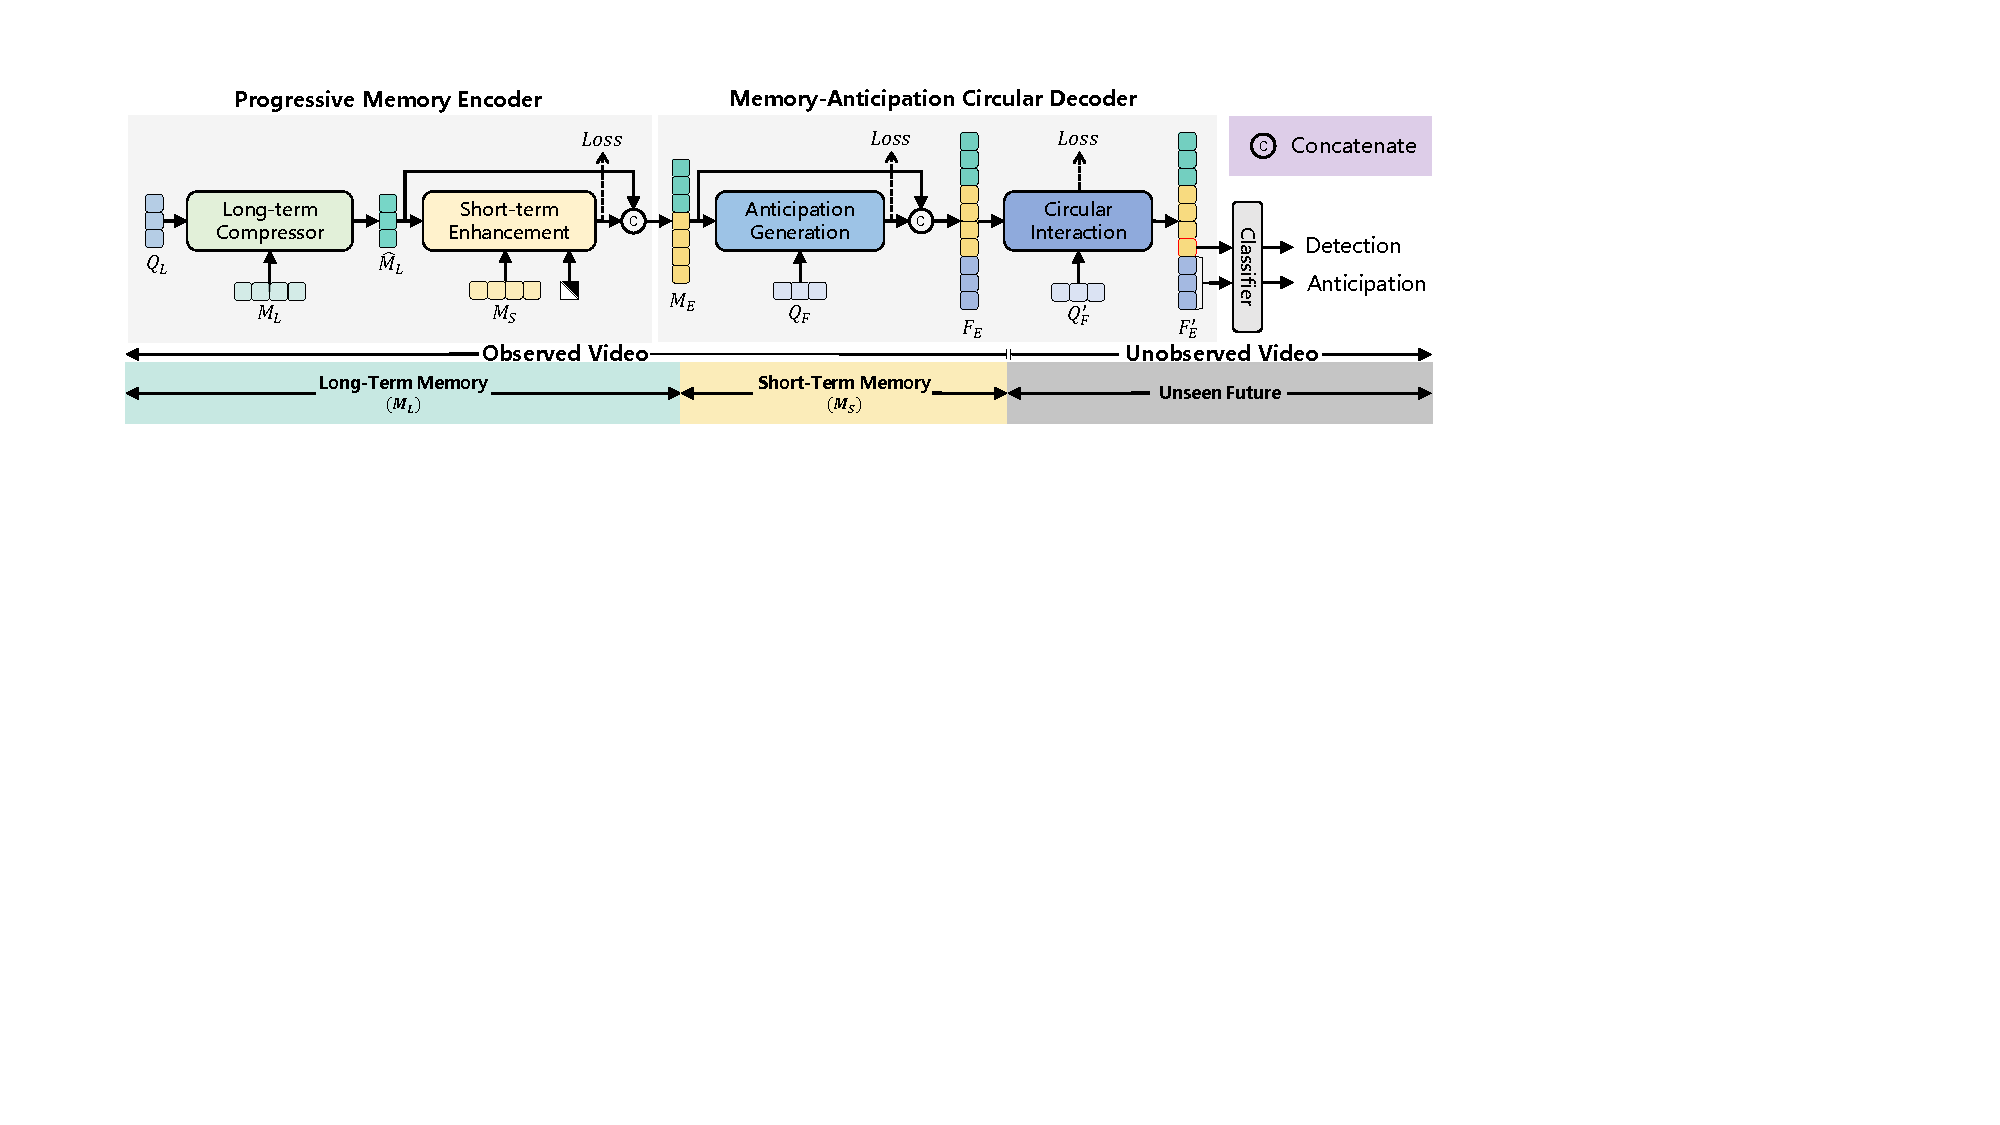
\includegraphics[width=1\textwidth]{images/Framework_new.pdf}
    \vspace{-2em}
    \caption{\textbf{MAT architecture.} We first divide the temporal sequence into long-term and short-term memories. 
    In \emph{Progessive Memory Encoder}, long-term memory queries $\mathbf{Q}_{L}$ progressively map the long-term to an abstract representation and be fed to the transformer decoder block to enhance the short-term memory. Then the \emph{Memory-Anticipation Circular Decoder} utilizes learnable queries $\mathbf{Q}_{F}$ and $\mathbf{Q}^{\prime}_{F}$ to perceive the future context and circularly updates the historical and future representation. Finally, a weight-shared classifier is adopted to output the classification scores of short-term and future for online action detection and anticipation.}
    \label{fig:framework}
\end{figure*}

Online action detection and anticipation share two key characteristics: the inability to perceive future representations, with information derived solely from historical context, and the goal of predicting actions after a certain time. 
Previous research has typically studied the model for each task in isolation~\cite{gatehub, colar} or trained and tested them separately~\cite{lstr,testra}, ignoring the potential benefits of leveraging their shared characteristics. We propose a novel unified framework, named MAT, to address this limitation, which allows us to train or infer both tasks simultaneously.



\textbf{Transformer for Video Understanding.} Transformers have proven successful in natural language processing \cite{transformer}, and researchers have shown increasing interest in its application to vision tasks \cite{vit, deit, swin, pvt, omnivore, li2023fb}. Several methods have been proposed to use transformers for temporal modeling in video-related tasks~\cite{vivit, longformer, videollm, cpmt, li2022uniformerv2, li2023unmasked, TadTR, linformer, wang2022internvideo, vidtr}.
Timesformer~\cite{timesformer} proposes divided attention to capture spatial and temporal information for action recognition separately. 
MViT~\cite{mvit} builds a feature hierarchy by progressively expanding channel capacity and reducing video spatial-temporal resolution. Actionformer~\cite{actionformer} adopts the transformer architecture with local attention for temporal action localization. 
TubeDETR~\cite{tubedetr} tackles video grounding with an encoder-decoder transformer-based architecture to efficiently encode spatial and multi-modal interactions.
Our MAT model is also built upon the transformer, utilizing its encoder and decoder architectures. We meticulously integrate the transformer blocks to implement our memory encoder and memory-anticipation circular decoder.
 



